\documentclass[]{article}
\usepackage{lmodern}
\usepackage{amssymb,amsmath}
\usepackage{ifxetex,ifluatex}
\usepackage{fixltx2e} % provides \textsubscript
\ifnum 0\ifxetex 1\fi\ifluatex 1\fi=0 % if pdftex
  \usepackage[T1]{fontenc}
  \usepackage[utf8]{inputenc}
\else % if luatex or xelatex
  \ifxetex
    \usepackage{mathspec}
  \else
    \usepackage{fontspec}
  \fi
  \defaultfontfeatures{Ligatures=TeX,Scale=MatchLowercase}
\fi
% use upquote if available, for straight quotes in verbatim environments
\IfFileExists{upquote.sty}{\usepackage{upquote}}{}
% use microtype if available
\IfFileExists{microtype.sty}{%
\usepackage{microtype}
\UseMicrotypeSet[protrusion]{basicmath} % disable protrusion for tt fonts
}{}
\usepackage[margin=1in]{geometry}
\usepackage{hyperref}
\hypersetup{unicode=true,
            pdftitle={Peer-graded Assignment: Course Project 1},
            pdfborder={0 0 0},
            breaklinks=true}
\urlstyle{same}  % don't use monospace font for urls
\usepackage{color}
\usepackage{fancyvrb}
\newcommand{\VerbBar}{|}
\newcommand{\VERB}{\Verb[commandchars=\\\{\}]}
\DefineVerbatimEnvironment{Highlighting}{Verbatim}{commandchars=\\\{\}}
% Add ',fontsize=\small' for more characters per line
\usepackage{framed}
\definecolor{shadecolor}{RGB}{248,248,248}
\newenvironment{Shaded}{\begin{snugshade}}{\end{snugshade}}
\newcommand{\KeywordTok}[1]{\textcolor[rgb]{0.13,0.29,0.53}{\textbf{#1}}}
\newcommand{\DataTypeTok}[1]{\textcolor[rgb]{0.13,0.29,0.53}{#1}}
\newcommand{\DecValTok}[1]{\textcolor[rgb]{0.00,0.00,0.81}{#1}}
\newcommand{\BaseNTok}[1]{\textcolor[rgb]{0.00,0.00,0.81}{#1}}
\newcommand{\FloatTok}[1]{\textcolor[rgb]{0.00,0.00,0.81}{#1}}
\newcommand{\ConstantTok}[1]{\textcolor[rgb]{0.00,0.00,0.00}{#1}}
\newcommand{\CharTok}[1]{\textcolor[rgb]{0.31,0.60,0.02}{#1}}
\newcommand{\SpecialCharTok}[1]{\textcolor[rgb]{0.00,0.00,0.00}{#1}}
\newcommand{\StringTok}[1]{\textcolor[rgb]{0.31,0.60,0.02}{#1}}
\newcommand{\VerbatimStringTok}[1]{\textcolor[rgb]{0.31,0.60,0.02}{#1}}
\newcommand{\SpecialStringTok}[1]{\textcolor[rgb]{0.31,0.60,0.02}{#1}}
\newcommand{\ImportTok}[1]{#1}
\newcommand{\CommentTok}[1]{\textcolor[rgb]{0.56,0.35,0.01}{\textit{#1}}}
\newcommand{\DocumentationTok}[1]{\textcolor[rgb]{0.56,0.35,0.01}{\textbf{\textit{#1}}}}
\newcommand{\AnnotationTok}[1]{\textcolor[rgb]{0.56,0.35,0.01}{\textbf{\textit{#1}}}}
\newcommand{\CommentVarTok}[1]{\textcolor[rgb]{0.56,0.35,0.01}{\textbf{\textit{#1}}}}
\newcommand{\OtherTok}[1]{\textcolor[rgb]{0.56,0.35,0.01}{#1}}
\newcommand{\FunctionTok}[1]{\textcolor[rgb]{0.00,0.00,0.00}{#1}}
\newcommand{\VariableTok}[1]{\textcolor[rgb]{0.00,0.00,0.00}{#1}}
\newcommand{\ControlFlowTok}[1]{\textcolor[rgb]{0.13,0.29,0.53}{\textbf{#1}}}
\newcommand{\OperatorTok}[1]{\textcolor[rgb]{0.81,0.36,0.00}{\textbf{#1}}}
\newcommand{\BuiltInTok}[1]{#1}
\newcommand{\ExtensionTok}[1]{#1}
\newcommand{\PreprocessorTok}[1]{\textcolor[rgb]{0.56,0.35,0.01}{\textit{#1}}}
\newcommand{\AttributeTok}[1]{\textcolor[rgb]{0.77,0.63,0.00}{#1}}
\newcommand{\RegionMarkerTok}[1]{#1}
\newcommand{\InformationTok}[1]{\textcolor[rgb]{0.56,0.35,0.01}{\textbf{\textit{#1}}}}
\newcommand{\WarningTok}[1]{\textcolor[rgb]{0.56,0.35,0.01}{\textbf{\textit{#1}}}}
\newcommand{\AlertTok}[1]{\textcolor[rgb]{0.94,0.16,0.16}{#1}}
\newcommand{\ErrorTok}[1]{\textcolor[rgb]{0.64,0.00,0.00}{\textbf{#1}}}
\newcommand{\NormalTok}[1]{#1}
\usepackage{graphicx,grffile}
\makeatletter
\def\maxwidth{\ifdim\Gin@nat@width>\linewidth\linewidth\else\Gin@nat@width\fi}
\def\maxheight{\ifdim\Gin@nat@height>\textheight\textheight\else\Gin@nat@height\fi}
\makeatother
% Scale images if necessary, so that they will not overflow the page
% margins by default, and it is still possible to overwrite the defaults
% using explicit options in \includegraphics[width, height, ...]{}
\setkeys{Gin}{width=\maxwidth,height=\maxheight,keepaspectratio}
\IfFileExists{parskip.sty}{%
\usepackage{parskip}
}{% else
\setlength{\parindent}{0pt}
\setlength{\parskip}{6pt plus 2pt minus 1pt}
}
\setlength{\emergencystretch}{3em}  % prevent overfull lines
\providecommand{\tightlist}{%
  \setlength{\itemsep}{0pt}\setlength{\parskip}{0pt}}
\setcounter{secnumdepth}{0}
% Redefines (sub)paragraphs to behave more like sections
\ifx\paragraph\undefined\else
\let\oldparagraph\paragraph
\renewcommand{\paragraph}[1]{\oldparagraph{#1}\mbox{}}
\fi
\ifx\subparagraph\undefined\else
\let\oldsubparagraph\subparagraph
\renewcommand{\subparagraph}[1]{\oldsubparagraph{#1}\mbox{}}
\fi

%%% Use protect on footnotes to avoid problems with footnotes in titles
\let\rmarkdownfootnote\footnote%
\def\footnote{\protect\rmarkdownfootnote}

%%% Change title format to be more compact
\usepackage{titling}

% Create subtitle command for use in maketitle
\newcommand{\subtitle}[1]{
  \posttitle{
    \begin{center}\large#1\end{center}
    }
}

\setlength{\droptitle}{-2em}

  \title{Peer-graded Assignment: Course Project 1}
    \pretitle{\vspace{\droptitle}\centering\huge}
  \posttitle{\par}
    \author{}
    \preauthor{}\postauthor{}
    \date{}
    \predate{}\postdate{}
  

\begin{document}
\maketitle

This is an R Markdown document for ``Course Project 1'' of
``Reproducible Research'' in Coursera.

\subsection{1. Code for reading in the dataset and/or processing the
data}\label{code-for-reading-in-the-dataset-andor-processing-the-data}

Initialization, reading dataset and additional preparation for the next
operations.

\begin{Shaded}
\begin{Highlighting}[]
\NormalTok{url <-}\StringTok{ "https://d396qusza40orc.cloudfront.net/repdata%2Fdata%2Factivity.zip"}
\NormalTok{zipfile <-}\StringTok{ "activity.zip"}
\NormalTok{datafile <-}\StringTok{ "activity.csv"}
\ControlFlowTok{if}\NormalTok{ (}\OperatorTok{!}\KeywordTok{file.exists}\NormalTok{(zipfile)) }\KeywordTok{download.file}\NormalTok{(url, zipfile)}
\ControlFlowTok{if}\NormalTok{ (}\OperatorTok{!}\KeywordTok{file.exists}\NormalTok{(datafile)) }\KeywordTok{unzip}\NormalTok{(zipfile)}
\ControlFlowTok{if}\NormalTok{ (}\OperatorTok{!}\KeywordTok{exists}\NormalTok{(}\StringTok{"da"}\NormalTok{)) da <-}\StringTok{ }\KeywordTok{read.csv}\NormalTok{(datafile)}

\NormalTok{da}\OperatorTok{$}\NormalTok{weekday <-}\StringTok{ }\KeywordTok{weekdays}\NormalTok{(}\KeywordTok{as.Date}\NormalTok{(da}\OperatorTok{$}\NormalTok{date))}
\NormalTok{da}\OperatorTok{$}\NormalTok{date2 <-}\StringTok{ }\KeywordTok{as.POSIXct}\NormalTok{(da}\OperatorTok{$}\NormalTok{date, }\DataTypeTok{format=}\StringTok{"%Y-%m-%d"}\NormalTok{)}
\NormalTok{da}\OperatorTok{$}\NormalTok{time2 <-}\StringTok{ }\KeywordTok{as.POSIXct}\NormalTok{(}\KeywordTok{formatC}\NormalTok{(da}\OperatorTok{$}\NormalTok{interval,}\DataTypeTok{width=}\DecValTok{4}\NormalTok{,}\DataTypeTok{flag=}\StringTok{"0"}\NormalTok{), }\DataTypeTok{format=}\StringTok{"%H%M"}\NormalTok{)}
\end{Highlighting}
\end{Shaded}

\subsection{2. Histogram of the total number of steps taken each
day}\label{histogram-of-the-total-number-of-steps-taken-each-day}

You can see the histogram of total numer of steps taken each day.The
most frequent step range is between 10,000 and 15,000. Also the curve
looks like normal distribution. Not so often over 20,000 steps. The R
script is simple using ``tapply()'' for ``step'' and ``date''.

\begin{Shaded}
\begin{Highlighting}[]
\NormalTok{totalStepDay<-}\KeywordTok{tapply}\NormalTok{(da}\OperatorTok{$}\NormalTok{step, da}\OperatorTok{$}\NormalTok{date, sum, }\DataTypeTok{rm.na=}\OtherTok{TRUE}\NormalTok{)}
\KeywordTok{hist}\NormalTok{(totalStepDay, }\DataTypeTok{xlab=}\StringTok{"steps"}\NormalTok{, }
     \DataTypeTok{main=}\StringTok{"Total number of steps taken each day"}\NormalTok{)}
\end{Highlighting}
\end{Shaded}

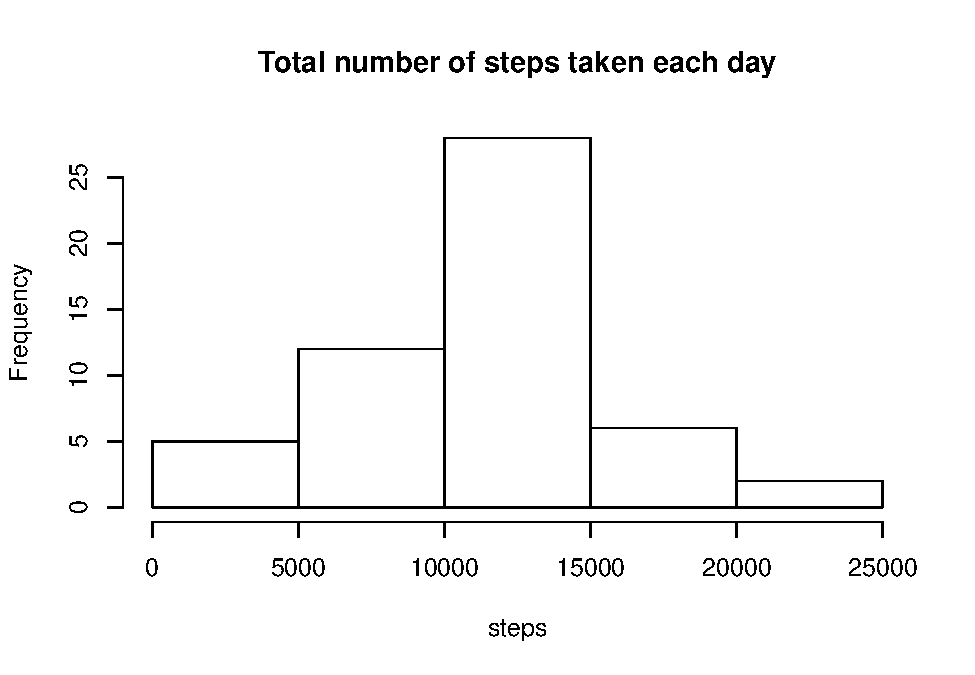
\includegraphics{PA1_template_files/figure-latex/total-1.pdf}

\subsection{3. Mean and median number of steps taken each
day}\label{mean-and-median-number-of-steps-taken-each-day}

Mean and median number of steps taken each day are
1.0767\times 10\^{}\{4\} and 10766. The median is rounded off using
``round()''.

\subsection{4. Time series plot of the average number of steps
taken}\label{time-series-plot-of-the-average-number-of-steps-taken}

Here are the R script and chart to show the average number of steps for
each interval. The script was cleaned up the activity data, and the
average steps were plotted for each 5-minute. The intervals are
transformed into actual time in advance. Many steps were obseved around
9:00AM because of commuting time probably.

\begin{Shaded}
\begin{Highlighting}[]
\NormalTok{da.tidy <-}\StringTok{ }\NormalTok{da[}\OperatorTok{!}\KeywordTok{is.na}\NormalTok{(da}\OperatorTok{$}\NormalTok{steps),]}
\NormalTok{meanInt<-}\KeywordTok{aggregate}\NormalTok{(da.tidy}\OperatorTok{$}\NormalTok{steps, }\DataTypeTok{by=}\KeywordTok{list}\NormalTok{(da.tidy}\OperatorTok{$}\NormalTok{time2), mean)}
\KeywordTok{names}\NormalTok{(meanInt)<-}\KeywordTok{c}\NormalTok{(}\StringTok{"interval"}\NormalTok{, }\StringTok{"steps"}\NormalTok{)}
\KeywordTok{plot}\NormalTok{(meanInt}\OperatorTok{$}\NormalTok{interval, meanInt}\OperatorTok{$}\NormalTok{steps, }\DataTypeTok{type=}\StringTok{"l"}\NormalTok{, }\DataTypeTok{xlab=}\StringTok{"interval"}\NormalTok{,}
     \DataTypeTok{ylab=}\StringTok{"mean of steps"}\NormalTok{, }\DataTypeTok{main=}\StringTok{"Average number of steps"}\NormalTok{)}
\end{Highlighting}
\end{Shaded}

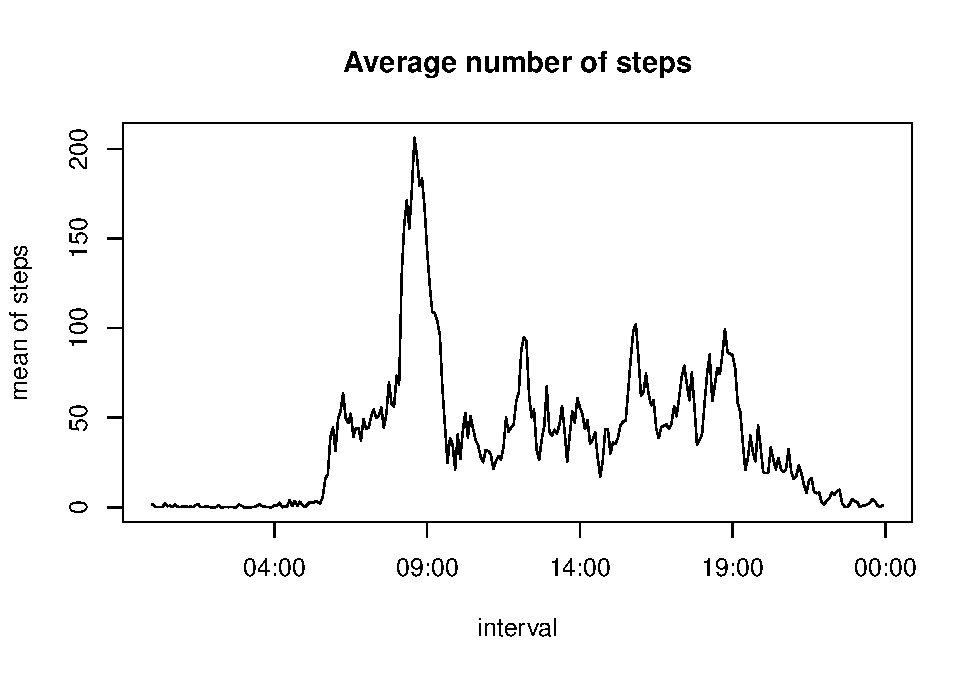
\includegraphics{PA1_template_files/figure-latex/unnamed-chunk-3-1.pdf}

\subsection{5. The 5-minute interval that, on average, contains the
maximum number of
steps}\label{the-5-minute-interval-that-on-average-contains-the-maximum-number-of-steps}

\begin{Shaded}
\begin{Highlighting}[]
\NormalTok{maxInt<-}\KeywordTok{aggregate}\NormalTok{(da.tidy}\OperatorTok{$}\NormalTok{steps, }\DataTypeTok{by=}\KeywordTok{list}\NormalTok{(da.tidy}\OperatorTok{$}\NormalTok{interval), max)}
\NormalTok{p.max<-}\KeywordTok{max}\NormalTok{(maxInt[,}\DecValTok{2}\NormalTok{])}
\end{Highlighting}
\end{Shaded}

The 5-minute interval that, on average, contains the maximum number of
steps is 806.

\subsection{6. Code to describe and show a strategy for imputing missing
data}\label{code-to-describe-and-show-a-strategy-for-imputing-missing-data}

\begin{Shaded}
\begin{Highlighting}[]
\NormalTok{p.missing<-}\KeywordTok{nrow}\NormalTok{(da[}\KeywordTok{is.na}\NormalTok{(da}\OperatorTok{$}\NormalTok{steps),])}
\end{Highlighting}
\end{Shaded}

The number of imputing missing data, specified as ``NA''``, is 2304.

\subsection{7. Histogram of the total number of steps taken each day
after missing values are
imputed}\label{histogram-of-the-total-number-of-steps-taken-each-day-after-missing-values-are-imputed}

In comparison with the previous histogram shown in \#3, this is total
number of steps taken each day after missing values are imputed. That
means all ``NA'' are taked into account. There are very small difference
between them.

\begin{Shaded}
\begin{Highlighting}[]
\NormalTok{totalStepDay<-}\KeywordTok{tapply}\NormalTok{(da}\OperatorTok{$}\NormalTok{step, da}\OperatorTok{$}\NormalTok{date, sum)}
\KeywordTok{hist}\NormalTok{(totalStepDay, }\DataTypeTok{xlab=}\StringTok{"steps"}\NormalTok{, }
     \DataTypeTok{main=}\StringTok{"Total number of steps each day after missing values are imputed"}\NormalTok{)}
\end{Highlighting}
\end{Shaded}

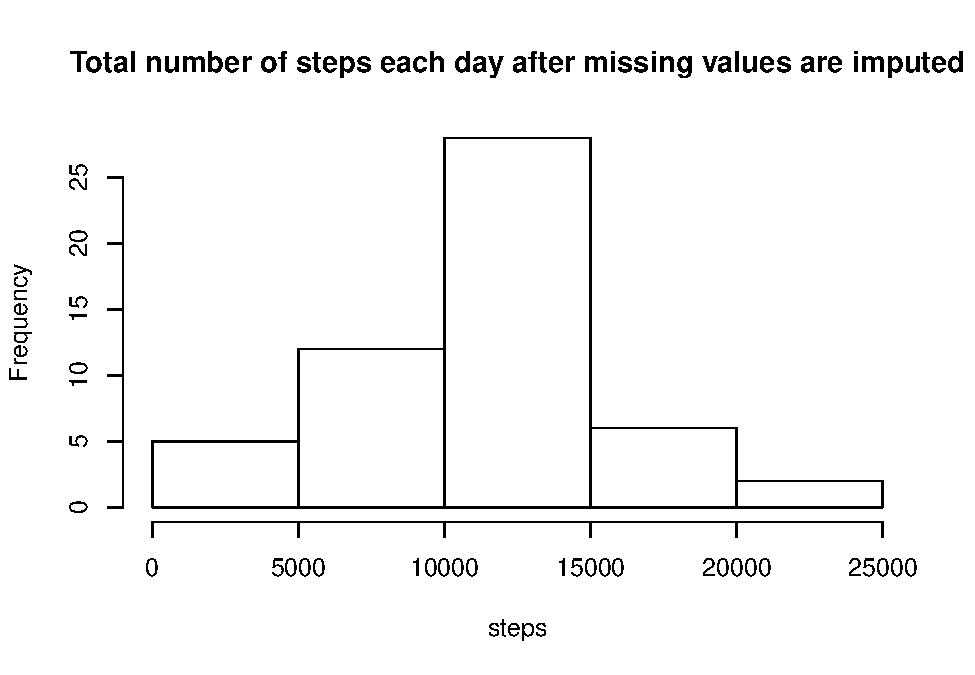
\includegraphics{PA1_template_files/figure-latex/unnamed-chunk-6-1.pdf}

\subsection{8. Panel plot comparing the average number of steps taken
per 5-minute interval across weekdays and
weekends}\label{panel-plot-comparing-the-average-number-of-steps-taken-per-5-minute-interval-across-weekdays-and-weekends}

In comparison to \#4, here are the R script and chart to show the
average number of steps for each interval on weekends and weekdays. We
can identify that the activity in the morning of weekdays was very high.
Also the commuting timing in the morning may be much more accurate that
that of in the evening.

\begin{Shaded}
\begin{Highlighting}[]
\NormalTok{da.tidy.we<-}\KeywordTok{subset}\NormalTok{(da.tidy, da.tidy}\OperatorTok{$}\NormalTok{weekday}\OperatorTok{==}\StringTok{"Saturday"}\OperatorTok{|}
\StringTok{                            }\NormalTok{da.tidy}\OperatorTok{$}\NormalTok{weekday}\OperatorTok{==}\StringTok{"Sunday"}\NormalTok{)}
\NormalTok{da.tidy.wd<-}\KeywordTok{subset}\NormalTok{(da.tidy, da.tidy}\OperatorTok{$}\NormalTok{weekday}\OperatorTok{!=}\StringTok{"Saturday"}\OperatorTok{&}
\StringTok{                            }\NormalTok{da.tidy}\OperatorTok{$}\NormalTok{weekday}\OperatorTok{!=}\StringTok{"Sunday"}\NormalTok{)}

\NormalTok{meanIntwe<-}\KeywordTok{aggregate}\NormalTok{(da.tidy.we}\OperatorTok{$}\NormalTok{steps, }\DataTypeTok{by=}\KeywordTok{list}\NormalTok{(da.tidy.we}\OperatorTok{$}\NormalTok{time2), mean)}
\NormalTok{meanIntwd<-}\KeywordTok{aggregate}\NormalTok{(da.tidy.wd}\OperatorTok{$}\NormalTok{steps, }\DataTypeTok{by=}\KeywordTok{list}\NormalTok{(da.tidy.wd}\OperatorTok{$}\NormalTok{time2), mean)}
\KeywordTok{names}\NormalTok{(meanIntwe)<-}\KeywordTok{c}\NormalTok{(}\StringTok{"interval"}\NormalTok{, }\StringTok{"steps"}\NormalTok{)}
\KeywordTok{names}\NormalTok{(meanIntwd)<-}\KeywordTok{c}\NormalTok{(}\StringTok{"interval"}\NormalTok{, }\StringTok{"steps"}\NormalTok{)}
\NormalTok{par.old<-}\KeywordTok{par}\NormalTok{(}\DataTypeTok{no.readonly=}\NormalTok{T)}
\KeywordTok{par}\NormalTok{(}\DataTypeTok{mfrow=}\KeywordTok{c}\NormalTok{(}\DecValTok{1}\NormalTok{,}\DecValTok{2}\NormalTok{))}
\KeywordTok{plot}\NormalTok{(meanIntwe}\OperatorTok{$}\NormalTok{interval, meanIntwe}\OperatorTok{$}\NormalTok{steps, }\DataTypeTok{type=}\StringTok{"l"}\NormalTok{, }\DataTypeTok{ylim=}\KeywordTok{c}\NormalTok{(}\DecValTok{0}\NormalTok{,}\DecValTok{250}\NormalTok{),}
     \DataTypeTok{xlab=}\StringTok{"interval"}\NormalTok{, }\DataTypeTok{ylab=}\StringTok{"mean of steps"}\NormalTok{,}
     \DataTypeTok{main=}\StringTok{"average steps, weekends"}\NormalTok{)}
\KeywordTok{plot}\NormalTok{(meanIntwd}\OperatorTok{$}\NormalTok{interval, meanIntwd}\OperatorTok{$}\NormalTok{steps, }\DataTypeTok{type=}\StringTok{"l"}\NormalTok{, }\DataTypeTok{ylim=}\KeywordTok{c}\NormalTok{(}\DecValTok{0}\NormalTok{,}\DecValTok{250}\NormalTok{),}
     \DataTypeTok{xlab=}\StringTok{"interval"}\NormalTok{, }\DataTypeTok{ylab=}\StringTok{"mean of steps"}\NormalTok{,}
     \DataTypeTok{main=}\StringTok{"average steps, weekdays"}\NormalTok{)}
\end{Highlighting}
\end{Shaded}

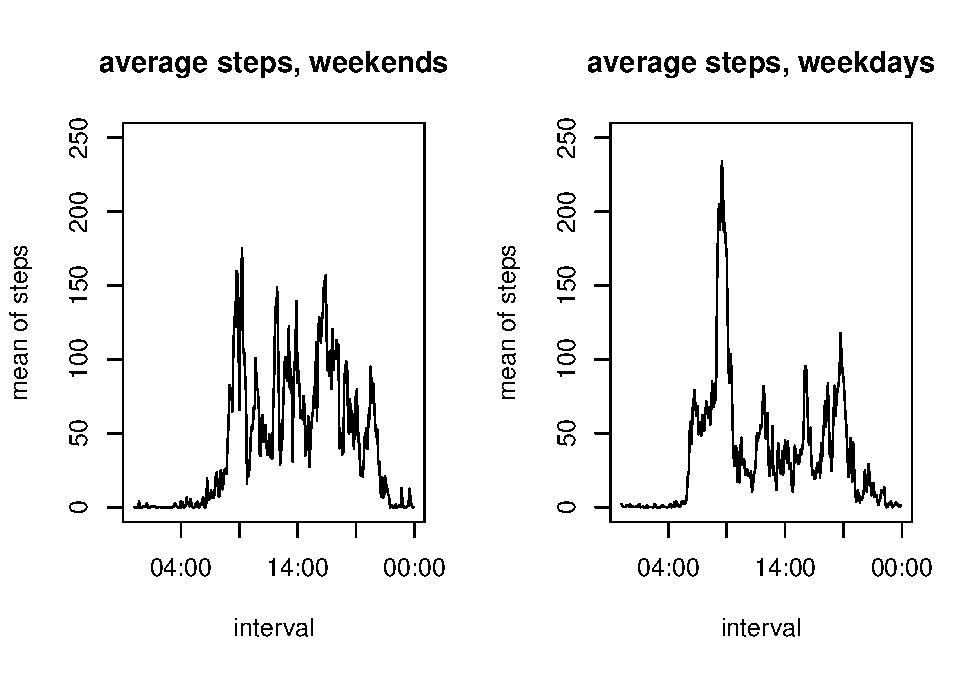
\includegraphics{PA1_template_files/figure-latex/unnamed-chunk-7-1.pdf}

\begin{Shaded}
\begin{Highlighting}[]
\KeywordTok{par}\NormalTok{(par.old)}
\end{Highlighting}
\end{Shaded}


\end{document}
